\section{Vector Space}
 
\begin{defn}[Vector Space]
 A vector space (or linear space) $V$ over a $Field$ $\mathcal{F}$ consists of a set on which two operations (called addition and scalar multiplication, respectively) are defined so that for each pair of elements $x, y$, in $V$ there is a unique element $x+y$ in $V$, and for each element a in F and each element $x$ in $V$ there is a unique element $ax$ in $V$, such that the following conditions hold.
\end{defn} 

\subsection*{\S\ Subspace }

\begin{defn}[Subspace]
	A subset $W$ of a vector space $V$ over a field $\mathbb{F}$ is called a subspace of $W$ if $W$ is a vector space over $\mathrm{F}$ with the operations of addition and scalar multiplication defined on $W$.
	
\end{defn}



\begin{rmk*}
	Trivial subspaces of a vector space $V$, namely $V$ itself and $\{0\}$. Note that empty set $\phi$ is not a vector space, since it does not contains a zero vector.
\end{rmk*}

\begin{thm}% thm 1.3
Let V be a vector space and W a subset of V. Then W is a subspace of V if and only if the following three conditions hold for the operations defined in V.
\\
(a)\ \ $0 \in W.$ \\
(b)\ \ $x+y \in W$ whenever $x \in W$ and $y \in W.$ \\
(c)\ \ $cx \in W$ whenever $c \in \mathrm{F}$ and $x \in W.$ \\

\end{thm}



\begin{cor} % ex 1.3.18
	Let $W$ be a subset of vector space $V$. $W$ is a subspace of $V$ if and only if $0\in W$ and $ax+y \in W$ whenever $a \in F$ and, $ x,y \in W$.
\end{cor}

\begin{proof}
	($\Rightarrow$) Since W is a subspace $\implies 0\in W$ , $ ax\in W $ for $a\in\mathcal{F}$ and $ax , y \in W \implies ax+y \in W$.
	($\Leftarrow$) $0\in W$. Since $ax+y\in W$, $a\in \mathcal{F}$, take $a= 1\implies x+y \in W$, and also $\because 0\in W,$ take $y=0\implies ax\in W$, for $a \in \mathcal{F}$. Hence, W isa subspace.   
\end{proof}


\begin{thm} % thm 1.4
 Any intersection of subspaces of a vector space $W$ is a subspace of $V$.
\end{thm}




\begin{thm} % ex 1.3.19
	Let $W_1$ and $W_2$ be subspaces of a vector space $V$, then $W_1 \cup W_2$ is a subspace of $V$ if and only if $W_1 \subseteq W_2$ or $W_2 \subseteq W_1$. 
\end{thm}

\begin{proof}
	Suppose $W_{1} \cup W_{2}$ is a subspace of $V$, we assume that $W_{1} \nsubseteq W_{2}$ and $W_{2} \nsubseteq W_{1}$. Let $x \in W_{1} \backslash W_{2}$ , $y \in W_{2} \backslash W_{1}$, then $x+y \in W_{1}$ or $W_{2}$, say $W_{1}$. But $y=(x+y)-x \in W_{1}$, which is a contradiction. So we have $W_{1} \subseteq W_{2}$ or $W_{2} \subseteq W_{1}$. Conversely is trivial.
\end{proof}


\begin{defn}
	If $S_1$ and $S_2$ are nonempty subsets of a vector space $V$, then the sum of $S_1$ and $S_2$, denoted $S_1 + S_2$, is the set $\{x+y:x \in S_1$ and $y\in S_2\}$.
\end{defn}

\begin{thm} % ex 1.3.23(a)(b)
	Let $W_1$ and $W_2$ be subspaces of a vector space $V$.
	\begin{itemize}
		\item[(a)] $W_1 + W_2$ is a subspace of $V$ that contains both $W_1$ and $W_2$.
		\item[(b)] Any subspace of V that contains both $W_1$ and $W_2$ must also contain $W_1 + W_2$. 
	\end{itemize}
\end{thm}
\begin{proof}
	To prove $(a)$, we first show that $W_{1}+W_{2}$ is a subspace of $V$. Clearly, $0=0+0 \in W_{1}+W_{2}$. Let $x=x_{1}+x_{2}$, $y=y_{1}+y_{2}$, $c \in \mathbb{F}$

$cx+y=c(x_{1}+x_{2})+(y_{1}+y_{2})=(cx_{1}+y_{1})+(cx_{2}+y_{2}) \in W_{1}+W_{2}$

By corrolary 1.1.1, $W_{1}+W_{2}$ is a subspace of $V$.

Then we show that $W_{1}, W_{2} \subseteq W_{1}+W_{2}$. $\forall x \in W_{1} y \in W_{2}$, $x=x+0 \in W_{1}+W_{2}$, $y=0+y \in W_{1}+W_{2}$, we have $W_{1}, W_{2} \subseteq W_{1}+W_{2}$.

To prove $(b)$, Let $W$ be a subspace of $V$ contains both $W_{1}$ and $W_{2}$, then $\forall x \in W_{1} , y \in W_{2}$, $x+y \in W_{1}+W_{2}$. Thus $W_{1}+W_{2} \subseteq W$. 
\end{proof}
%\begin{proof}
	To prove $(a)$, we first show that $W_{1}+W_{2}$ is a subspace of $V$. Clearly, $0=0+0 \in W_{1}+W_{2}$. Let $x=x_{1}+x_{2}$, $y=y_{1}+y_{2}$, $c \in \mathbb{F}$

$cx+y=c(x_{1}+x_{2})+(y_{1}+y_{2})=(cx_{1}+y_{1})+(cx_{2}+y_{2}) \in W_{1}+W_{2}$

By corrolary 1.1.1, $W_{1}+W_{2}$ is a subspace of $V$.

Then we show that $W_{1}, W_{2} \subseteq W_{1}+W_{2}$. $\forall x \in W_{1} y \in W_{2}$, $x=x+0 \in W_{1}+W_{2}$, $y=0+y \in W_{1}+W_{2}$, we have $W_{1}, W_{2} \subseteq W_{1}+W_{2}$.

To prove $(b)$, Let $W$ be a subspace of $V$ contains both $W_{1}$ and $W_{2}$, then $\forall x \in W_{1} , y \in W_{2}$, $x+y \in W_{1}+W_{2}$. Thus $W_{1}+W_{2} \subseteq W$. 
\end{proof}


\begin{defn}[Direct Sum] A vector space $V$ is called the direct sum of $W_1$ and $W_2$ if $W_1$ and $W_2$ are subspaces of V such that $W_1 \cap W_2 = \{0\}$ and $W_1 + W_2 = V$. We denote that $V$ is the direct sum of $W_1$ and $W_2$ by writing $V = W_1 \oplus W_2$.
\end{defn}

\begin{thm} % ex 1.3.30
	Let $W_1$ and $W_2$ be subspaces of a vector space $V$. $V$ is the direct sum of $W_1$ and $W_2$ i.e. $$ V = W_1 \oplus W_2 $$ if and only if each vector in $V$ can be uniquely written as $x_1 + x_2$, where $x_1 \in W_1$ and $x_2 \in W_2$
\end{thm}

\begin{solution}
			Suppose that we can write $v = x_1 + x_2 = y_1 + y_2$ with $x_1,y_1 \in W_1$ and $x_2,y_2 \in W_2$. Since $x_1 + x_2 = y_1 + y_2$ and $W_1,W_2$ are subsapces of a vector space $V$, so $x_1 - y_1 = x_2 - y_2 \in W_1 \cap W_2$. As $V =  W_1 \oplus W_2$, $x_1 - y_1 = x_2 - y_2 = \{0\}$, that is, $x_1 = y_1$ and $x_2 = y_2$. Hence it is a unique representation. Conversely, suppose that the condition holds. We claim that $V = W_1 + W_2$ and $W_1 \cap W_2 = \{0\}$. Since $W_1 + W_2$ is the smallest subspace of $V$, so $W_1 + W_2 \subseteq V$. By assumption, it is clear to get that $V \subseteq W_1 + W_2$. This proves $V = W_1 + W_2$. Since $W_1,W_2$ are subspaces of $V$, so $0 \in W_1$ and $0 \in W_2$. Let $v$ be a vector in $W_1 \cap W_2$. From the uniqueness of decomposition and $v = 0 + v = v + 0$, it implies that $v = 0$. This proves $W_1 \cap W_2 = \{0\}$. In conclusion, $V = W_1 \oplus W_2$.
		\end{solution}


\subsection*{\S\ Linear Combinations and Bases}

\begin{defn}[Linearly Dependent]
	A subset $S$ of a vector space $W$ is called linearly dependent if there exist a finite number of distinct vectors $u_1, u_2, . . . , u_n$ in $S$ and scalars $a_1,a_2,...,a_n$, not all zero, such that 
	
		$$a_1u_1 + a_2u_2 +\cdots +a_nu_n = 0 .$$
	
In this case we also say that the vectors of $S$ are linearly dependent.

\end{defn}

\begin{defn}[Linearly Independent]
	A subset $S$ of a vector space that is not linearly dependent is called linearly independent. As before, we also say that the vectors of $S$ are linearly independent.
\end{defn}

\begin{rmk*}$ $
	\begin{enumerate}
		\item The empty set is linearly independent, for linearly dependent sets must be nonempty.
		\item A set consisting of a single nonzero vector is linearly independent. For if $\{u\}$ is linearly dependent, then $au = 0$ for some nonzero scalar $a$. Thus
			$$ u = a^{-1}(au) = a^{-1} 0 = 0 $$
		\item A set is linearly independent if and only if the only representations of $0$ as linear combinations of its vectors are trivial representations.
	\end{enumerate}
\end{rmk*}

\begin{thm}% thm 1.6
	Let $V$ be a vector space, and let $S_1 \subseteq S_2 \subseteq V$. If $S_1$ is linearly dependent, then $S_2$ is linearly dependent.
\end{thm}

\begin{proof}
	Since $S_1 = \{u_1 , \cdots,u_m\}$ is linearly dependent i.e. $\exists\ a_1,\cdots,a_m \in \mathcal{F}$ are not all zero s.t. $$ a_1u_1+\cdots + a_mu_m = 0 \quad \quad(1)$$ Since $S_1 \subseteq S_2$ say $S_2 = S_1 \cup \{u_{m+1},\cdots,u_n\}$. Let $$b_1u_1 + \cdots+b_mu_m+b_{m+1}u_{m+1}+\cdots + b_{n}u_n = 0\ b_j\in\mathcal{F} ,  j= 1,2,3,\cdots $$ Now, we take $b_{m+1}=\cdots = b_{n}=0$ and by (1) there exists $a_1,\cdots,b_{n}$ are not all zeros. Hence, $S_2$ is linearly dependent.  
\end{proof}



\begin{cor}% thm 1.6 cor
	Let $S$ be a linearly independent subset of a vector space $V$, and let $v$ be a vector in $V$ that is not in $S$. Then $S \cup \{v\}$ is linearly dependent if and only if $v \in span(S)$.
\end{cor}

\begin{proof}
	Suppose $S \cup {v}$ is linear independent, then $\exists v_1, ... , v_n \in S \cup {v}$ such that $a_1u_1+...+a_nu_n = 0$ for some nonzero scalars $a_1, ... ,a_n$. Because $S$ is linear independent, say $u_1 = v$. We have $v = a_1^{-1}(-a_2u_2-...-a_nu_n)$, which is a linear combination of ${u_2,...,u_n}$. Thus $v \in span(S)$. Conversely, suppose $v \in span(S)$. Then $\exists v_1,...,v_n \in S$ and scalars $b_1,...,b_m$ such that $v=b_1v_1+...+b_mv_m$. Thus $0=b_1v_1+...+b_mv_m+(-1)v$ which means $S \cup {v}$ is linear independent.
\end{proof}


%\begin{thm}% thm 1.7
	%Let $S$ be a linearly independent subset of a vector space $V$, and let $v$ be a vector in $V$ that is not in $S$. Then $S \cup \{v\}$ is linearly dependent if and only if $v \in $ span($S$).
%\end{thm}

%\begin{proof}
	Let $\beta$ be a basis of $v$. Suppose $v=a_1u_1+...+a_nu_n=b_1u_1+...+b_nu_n$. We have $0=(a_1-b_1)u_1+...+(a_n-b_n)u_n$. Since $\beta$ is linear independent, we have $(a_1-b_1)=...=(a_n-b_n)$, hence $a_1=b_1,...,a_n=b_n$, which means $v$ is uniquely expressed as a linear combination of $\beta$. Conversely, suppose $v$ can be uniquely expressed as a linear combination of $\beta$. Clearly, $\beta$ generates $V$ and the representation of $0$ is unique. So if $0=a_1u_1+...+a_nu_n$, we have $a_1=...=a_n$. Thus $\beta$ is linear independent and is a basis of $V$.
\end{proof}


\begin{defn}[Basis]
A basis $\beta$ for a vector space $V$ is a linearly independent subset of $V$ that generates $V$. If $\beta$ is a basis for $V$, we also say that the vectors of $\beta$ form a basis for $V$.
		
\end{defn}

\begin{thm} % thm 1.8
	Let $V$ be a vector space and $\beta = \{u_1,u_2,...,u_n \}$ be a subset of $V$. Then $\beta$ is a basis for V if and only if each  $v\in$ V can be uniquely expressed as a linear combination of vectors of $\beta$, that is, can be expressed in the form

	$$ V = a_1u_1 + a_2u_2 + \cdots+ a_nu_n $$

for unique scalars $a_1, a_2, \cdots , a_n$.	
\end{thm}

\begin{proof}
	If $S= \emptyset$ or $S={0}$, then $V=\{0\}$ and $\emptyset$ is a subset of $S$ which is a basis of $V$. Otherwise $S$ contains a nonzero vector $\{u_1\}$. We continue choosing vectors $u_2,...,u_k \in S$ such that $\beta = \{u_1,...,u_k\}$ is linear independent and $\{u_1,...,u_k,v\}$ is linear dependent for some vector $v \in V \backslash S$. To show that $\beta$ is a basis, it suffices toshow that $\beta$ generates $V$. Let $v \in S$. If $v \in \beta$, then clearly $\beta \in span(S)$. If $v \in S \backslash \beta$, then we have $\beta \cup {v}$ is linear dependent. So $v \in span(\beta)$. Thus $S \subseteq span(\beta)$.
\end{proof}


\begin{thm} % thm 1.9
	If a vector space $V$ is generated by a finite set $S$, then some subset of $S$ is a basis for $V$. Hence $V$ has a finite basis.	
\end{thm}

\begin{proof}
	We prove it by mathematical induction on $m$. For $m=0$, $L = \emptyset$, so take $H=G$. Assume the theorem holds for some integer $m \geq 0$. For $ m+1 $, let $L = \{ v_1,...,v_{m+1} \}$ be a linear independent subset of $V$ containing $m+1$ vectors. Because $\{v_1,...,v_m\}$ is linear independent, so by the induction  hypothesis, we have $m \geq n$ and $\exists$ a subset $\{u_1,...,u_{n-m}\}$ of $G$ such that $\{v_1,...,v_m\} \cup \{u_1,...,u_{n-m}\}$  generates $v$. Thus $\exists$ scalars $a_1,...,a_m,b_1,...,b{n-m}$ such that $a_1v_1+...+a_mv_m+b_1u_1+...+b_{n-m}u_{n-m}=v_{m+1}$. We have $n-m>0$ and $v_{m+1}$ is a linear combination of $\{v_1,...,v_m\}$ which contradicts the assumption that $L$ is linear independent. Hence $n>m$ that is $n \geq m+1$. Moreover, say $b_1$ is nonzero, otherwise we obtain the same contradiction. We have $u_1 = (-b_1^{-1}a_1)v_1+...+(-b_1^{-1}a_m)v_m+(b_1^{-1})v_{m+1}+(-b_1^{-1}b_2)u_2+...+(-b_1^{-1}b_{n-m})u_n-m$. Let $H = \{u_2,...,u_{n-m}\}$. Then $u_1 \in span(L \cup H)$ and $v_1,...,v_m,u_2,...,u_{n-m} \in span(L \cup H)$, so $ \{v_1,...,v_m,u_1,...,u_{n-m} \} \subseteq span(L \cup H)$.  We have $span(L \cup H)=V$. Since $H$ is a subset of $G$  contains $(n-m)-1=n-(m+1)$ vectors. So by mathematical induction, we are done.
\end{proof}


\begin{thm}[Replacement Theorem] % thm 1.10
	Let $V$ be a vector space that is generated by a set $G$ containing exactly $n$ vectors, and let $L$ be a linearly independent subset of $V$ containing exactly $m$ vectors. Then $m \leq n$ and there exists a subset $H$ of $G$ containing exactly $n - m$ vectors such that $L \cup H$ generates $V$.
\end{thm}

\begin{proof}
	Let $dim(V)=n$. If $W=\{0\}$, then $W$ is finite-dimensional and $dim(W)=0 \leq n$. Otherwise, $W$ contains a nonzero vector $x_1$, so $\{_1\}$ is a linear independent set. We continue choosing vectors $x_1,...,x_k \in W$ such that ${x_1,...,x_k}$ is linear independent. This process must stop at $k \leq n$ and $\{x_1,...,x_k\}$ is linear independent and other vector in $W$ produces a linear dependent set. Hence it is a basis of $W$. Thus $dim(W)=k \leq n$. If $dim(W)=n$, a basis of $W$ is a linear independent subset of $V$ contains $n$ vectors, so a basis of $W$ is also a basis of $V$. Thus $W=V$.

\end{proof}


\begin{cor} % thm 1.10 cor1
	Let $V$ be a vector space having a finite basis. Then every basis for $V$ contains the same number of vectors.	
\end{cor}

%\redd{not yet}

\begin{defn}[Finite-Dimensional]
	A vector space is called finite-dimensional if it has a basis consisting of a finite number of vectors. The unique number of vectors
 in each basis for $V$ is called the dimension of $V$ and is denoted by $dim(V)$.
A vector space that is not finite-dimensional is called infinite-dimensional.
\end{defn}


\begin{cor}% thm 1.10 cor2
	Let $V$ be a vector space with dimension $n$.
	\begin{enumerate}
		\item Any finite generating set for $V$ contains at least n vectors, and a generating set for $V$ that contains exactly n vectors is a basis for $V$.
		\item Any linearly independent subset of $V$ that contains exactly n vectors is a basis for $V$.
		\item Every linearly independent subset of $V$ can be extended to a basis for $V$.
	\end{enumerate}
\end{cor}

%\redd{not yet}


% The figure is left to Jester
\begin{center}
		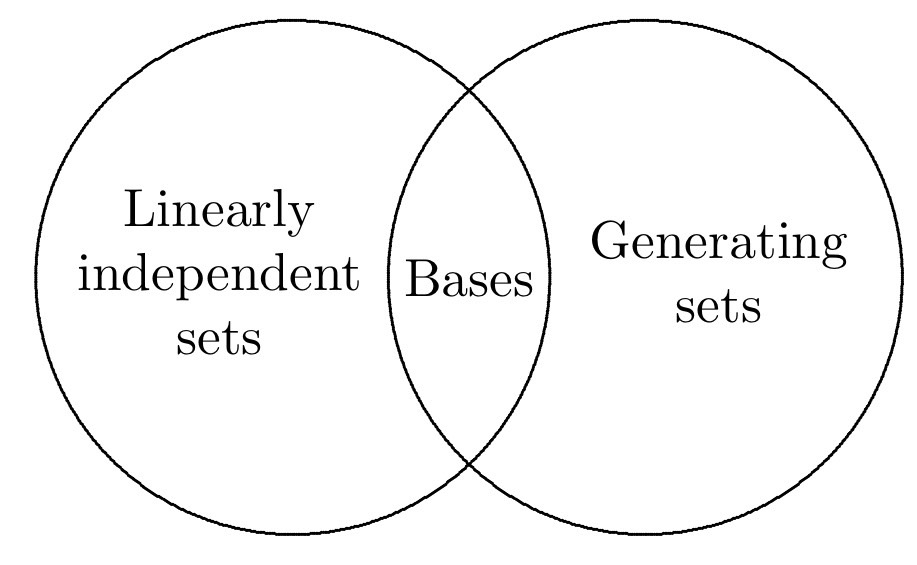
\includegraphics[scale = 0.25]{./figure/49.jpg}
\end{center}


\begin{thm} %thm 1.11
Let $W$ be a subspace of a finite-dimensional vector space $V$. Then $W$ is finite-dimensional and $\dim(W) \leq \dim(V)$. Moreover, if $\dim(W) = \dim(V)$, then $V = W$.
\end{thm}

\begin{proof}
	Since $V$ is a finite-dimensional vector space, say $\dim(V) = n$. If $W = \{0\}$, then $W$ is a finite-dimensional and $\dim(W) = 0 \leq n$. Otherwise, $W$ contains a nonzero vector $x_1$ ; so $\{x_1\}$ is linearly independent set. Continue choosing vectors, $x_1,\cdots,x_k $ in $W$ such that $S = \{x_1,\cdots,x_k\}$ is linearly independent. Since no linearly independent subset can contain more than $n$ vectors in $V$, therefore $S \cup \{v\}$ is linearly dependent for $\{v\}\in span(S)$ then by Thm 1.7 $S$ generates $W$. $S$ is a basis of $W \implies \dim(W) = k \leq n$. If $\dim(W) = n$, then a basis for $W$ is a linearly independent subset of $V$ containing $n$ vectors. By replacement theorem any linearly independent subset of $V$ contains exactly $n$ vectors is also a basis of $V$. Hence $V = W$.  
\end{proof}  


\begin{prop} % ex 1.6.22 
	Let $W_1$ and $W_2$ be subspaces of a finite-dimensional vector space $V$. $W_1 \subseteq W_2$ if and only if $\dim(W_1 \cap W_2) = \dim(W_1)$
\end{prop}

%\redd{not yet} The proof is too trivial


\begin{thm} % ex 1.6.23
Let $v_1, v_2, \cdots , v_k, v$ be vectors in a vector space $V$, and define $W_1 = span(\{v_1, v_2, \cdots , v_k\})$, and $W_2 = span(\{v_1, v_2, \cdots , v_k , v \})$.Then $v \in \mathrm{span}(W_1)$ if and only if $\dim(W_1) = \dim(W_2)$.
\end{thm}

%\redd{not yet}


\begin{rmk*}
	We may give an example for satisfying the conditions on above but $\dim(W_1) \neq \dim(W_2)$.
\end{rmk*}

%\begin{defn}[Direct Sum (Recall)]
%	A vector space $V$ is called the direct sum of $W_1$ and $W_2$ if $W_1$ and $W_2$ are subspaces of V such that $W_1 \cap W_2 = \{0\}$ and $W_1 + W_2 = V$. We denote that $V$ is the direct sum of $W_1$ and $W_2$ by writing $V = W_1 \oplus W_2$.
% \end{defn}

\begin{thm} % ex 1.6.29
Let $W_1$ and $W_2$ be finite-dimensional subspaces of a vector space $V$.
\begin{enumerate} 
	\item [(a)]Then the subspace $W_1 + W_2$ is finite-dimensional, and $$\dim(W_1 + W_2) = \dim(W_1) + \dim(W_2) - \dim(W_1 \cap W_2)$$
    \item [(b)]  Let $V = W_1 + W_2$. Deduce that $V$ is the direct sum of $W_1$ and $W_2$ if and only if $$\dim(V) = \dim(W_1) + \dim(W_2)$$
\end{enumerate}	
\end{thm}

\begin{proof}$ $

\begin{enumerate}
	\item[(a).] Let $\beta= \sett{u_1,u_2,\cdots,u_k}$ is a basis of $W_1 \cap W_2$ with $\dim(W_1) = k+m$, $\dim(W_2) = k+n$ and $\dim(W_1 \cap W_2) = k$ for $k,m,n \in \N$. Since $\beta \in W_1$ and $ \beta \in W_2$ by Replacement Theorem, every linearly independent subset of $V$ can be extended to a basis for $V$.
			
			$\exists~\beta_1 = \sett{u_1, u_2,\cdots, u_k , v_1,v_2 , \cdots,v_m}$ is a basis of $W_1$ and $\beta_2 = \sett{u_1, u_2,\cdots,u_k,w_1,w_2,\cdots,w_n}$ is a basis of $W_2$. Let $x \in W_1 + W_2$.
			
			\textbf{Claim.} $Span(\sett{u_1,\cdots,u_k,v_1,\cdots,v_m,w_1,\cdots,w_n}) = W_1 + W_2$
			
			$x = (a_1u_1 + a_2u_2 + \cdots + a_{k+1}v_1+a_{k+2}v_2 + \cdots + a_{k+m}v_m)+(b_1u_1+b_2u_2+\cdots+b_ku_k+b_{k+1}w_{1}+b_{k+2}w_2+\cdots+b_{k+n}w_n), a_i,b_j\in\mathcal{F}$ for $i ,j=1,2,\cdots$
			
			$=c_1u_1 + c_2u_2 + \cdots + c_ku_k + a_{k+1}v_1 + a_{k+2}v_2+\cdots + a_{k+m}v_m + b_{k+1}w_1 + b_{k+2} + \cdots + b_{k+n}w_n, c_1,c_2,\cdots,c_k \in \mathcal{F}\implies \forall~x \in W_1 + W_2 $ 
			
			$\therefore W_1 + W_2 \subseteq span(\sett{u_1,\cdots,u_k,v_1,\cdots,v_m,w_1,\cdots,w_n})$
			
			$\because W_1 + W_2$ is a subspace, any linear combination of $W_1 + W_2$'s subset are in $W_1 + W_2$
			
			$\therefore span(\sett{u_1,\cdots,u_k,v_1,\cdots,v_m,w_1,\cdots,w_n}) \in W_1 + W_2$
			
			$\therefore span(\sett{u_1,\cdots,u_k,v_1,\cdots,v_m,w_1,\cdots,w_n}) = W_1 + W_2$
			
			\textbf{Claim.} $\sett{u_1,\cdots,u_k,v_1,\cdots,v_m,w_1,\cdots,w_n}$ is linearly independent
			
			$\sum^k_{i=1}a_iu_i + \sum^m_{i=1}b_iv_i + \sum^n_{i=1}c_iw_i = 0$
			$\implies \sum^k_{i=1}a_iu_i + \sum^m_{i=1}b_iv_i = -\sum^n_{i=1}c_iw_i$
			
			$\because \sum^{k}_{i=1}a_iu_i + \sum^{m}_{i=1}b_iv_i \in W_1~,~ -\sum^n_{i=1}c_iw_i \in W_2$
			
			$\therefore \sum^k_{i=1}a_iu_i + \sum^m_{i=1}b_iv_i~,~-\sum^n_{i=1}c_iw_i \in W_1 \cap W_2$
			
			$\implies \exists~d_i \in \mathcal{F}, \sum^k_{i=1}a_iu_i + \sum^m_{i=1}b_iv_i = -\sum^n_{i=1}c_iw_i = \sum^k_{i=1}d_iu_i$
			
			$\because \beta_1 , \beta_2$ is linearly independent
			$\therefore -\sum^n_{i=1}c_iw_i = \sum^k_{i=1}d_iu_i$ only for scalars are all zeros.
			$\sum^k_{i=1}a_iu_i + \sum^m_{i=1}b_iv_i = 0$ only for scalars are all zero
			
			$\therefore \{u_1,\cdots,u_k,v_1,\cdots,v_m,w_1,\cdots,w_n\}$ is linearly independent

			$\therefore \sett{u_1,u_2,\cdots,u_k,v_1,v_2,\cdots,v_m,w_1,w_2,\cdots,w_n}$ is a basis of $W_1 + W_2$
			
			
			
			$\therefore$ dim($W_1 + W_2$) = $k+m+n$
			
			dim($W_1 + W_2$) = dim($W_1$) + dim($W_2$) + dim($W_1 \cap W_2$)
			
			\item [(b).] $W_1 \cap W_2 = \sett{0}$
			
			by Exercise 1.16.29(a), if $W_1$ and $W_2$ are finite-dimensional subspace of a vector space V, dim(V) = dim($W_1$) + dim($W_2$) - dim($W_1 \cap W_2$) = dim($W_1$) + dim($W_2$) - dim($\sett{0}$) = dim($W_1$) + dim($W_2$)


\end{enumerate} 			
						
	\end{proof}



\begin{thm} % ex 1.6.33
Let $W_1$ and $W_2$ be subspaces of a vector space $V$ such that $V = W_1 \oplus W_2$ if and only if there exist base $\beta_1$ , $\beta_2$ of $W_1$ , $W_2$, respectively such that $\beta_1 \cup \beta_2$ is a basis for $V$.
\end{thm}

\begin{proof}
	Let $\beta_1 = \sett{v_1,v_2,\cdots,v_n},v_1,v_2,\cdots,v_n \in W_1$,
		
		 $\beta_2 = \sett{u_1,u_2,\cdots,u_m},u_1,u_2,\cdots,u_m \in W_2$
		
		$W_1 + W_2 = \left\{\sum_{i=1}^n a_iv_i + \sum_{j=1}^{m}b_ju_j ~|~ a_1,\cdots,a_n,b_1,\cdots,b_m \in \mathcal{F}\,\right\} $
		\vspace*{0.2cm}
		
		\textbf{Claim : } $\spann{\beta_1 \cup \beta_2} \subseteq W_1 + W_2$
		
		let $x \in \spann{\beta_1 \cup \beta_2}~, x = a_1v_1 + a_2v_2 + \cdots + b_1u_1 + b_2u_2 + \cdots + b_mu_m$
		
		$\because W_1,W_2$ is a subspace of V $\therefore \sum^{n}_{i=1}a_iv_i \in W_1~,~ \sum^{m}_{i=1}b_iu_i \in W_2$
		
		$\therefore x \in W_1 + W_2,\spann{\beta_1 \cup \beta_2} \subseteq W_1 + W_2$
		
		\vspace*{0.3cm}
		\textbf{Claim.} $W_1 + W_2 \subseteq \spann{\beta_1 \cup \beta_2}$
		
		Let $x \in W_1 + W_2, x = (a_1v_1 + \cdots + a_nv_n) + (b_1u_1 + \cdots  + b_mu_m)$
		
		$\therefore x \in \spann{\beta_1 \cup \beta_2}$\ 
		$\therefore W_1 + W_2 \subseteq \spann{\beta_1 \cup \beta_2}$\ 
		$\therefore \spann{\beta_1 \cup \beta_2} = W_1 + W_2$

		
	    \vspace*{0.3cm}
		\textbf{Claim} ${\beta_1 \cup \beta_2}$ is linearly independent
		
		$\sum^n_{i=1}a_iv_1 + \sum^m_{j=1}b_ju_j = 0$ 
		$\implies\sum^n_{i_1}a_iv_i = -\sum^m_{j=1}b_ju_j$
		
		$\because \sum^n_{i=1}a_iv_i \in W_1~,~ -\sum^m_{j=1}b_ju_j \in W_2$ and $\sum^n_{i=1}a_iv_i~,~-\sum^m_{i=1}b_iu_i \in W_1 \cap W_2$ 
		
		$\because W_1 \cap W_2$ $\therefore \sum^n_{i=1}a_iv_i = -\sum^m_{j=1}b_ju_j = 0$ \ \ $\because \beta_1 , \beta_2$ is linearly independent
		
		$\therefore a_1 = \cdots = a_n = b_1=\cdots = b_m =0$ $\therefore \beta_1 \cup \beta_2$ is linearly independent
		
		$\therefore \beta_1 \cup \beta_2$ is a basis of V.

\end{proof}


\begin{thm} % ex 1.6.34
		\item If $W_1$ is any subspace of vector space of $V$, then there exists a subspace $W_2$ of $V$ such that $$ V = W_1 \oplus W_2 $$
\end{thm}
\begin{proof}
	let $\beta_1 = \sett{v_1,v_2,\cdots,v_m}$ and $\dim(V) = n$.
	By Corollary of Replacement Theorem, Every linearly independent subset of V can be extended to a basis for V then
		$\exists~\beta = \sett{v_1,v_2,\cdots,v_m,u_1,u_2,\cdots,u_{n-m}}$ is a basis of $V$. Let $W_2 = \text{span$(\{u_1,u_2,\cdots,u_{n-m}\})$}$
		$\because u_1,u_2,\cdots,u_{n-m} \in V,V$ is a vector space 
		
		by Thm 1.5, the span of any subset S of a vector space V is a subspace.
		
		$\therefore W_2$ is a subspace of V. Now we claim that $W_1 \cap W_2 = \{0\}$
		
		$\because W_1,W_2$ is a subspace of V $\therefore 0 \in W_1 , W_2$.
		Assume $\exists~r \in V$ and $ r \in W_1~,~ r \in W_2~,~ r \neq 0$.
		
		$$\begin{flalign*}
			r & =  a_1v_1 + a_2v_2 + \cdots + a_mv_m &\\
			& =  b_1u_1 + b_2u_2 + \cdots + b_{n-m}u_{n-m} &\\
			& =  c_1v_1 + \cdots + c_mv_m + d_1u_1 + \cdots + d_{n-m}u_{n-m}&
		\end{flalign*}$$
		
		$\implies
		\begin{cases}
			(c_1-a_1)v_1+\cdots+(c_m-a_m)v_m+d_1u_1+\cdots+d_{n-m}u_{n-m} = 0 \\
			c_1v_1 + \cdots + c_mv_m+(d_1-b_1)u_1 + \cdots + (d_{n-m}-b_{n-m})		
		\end{cases}$
		
		$\implies c_1 = a_1,c_2=a_2,\cdots,c_m=a_m,d_1=b_1,\cdots,d_{n-m} = b_{n-m}$
		
		$\Rightarrow r = r+r \Rightarrow r=0 \rightarrow\leftarrow $ $\therefore W_1 \cap W_2 = \{0\}$.
\end{proof}


         